\documentclass{article}
\usepackage[LGR,T1]{fontenc}
\usepackage[utf8]{inputenc}
\usepackage[greek, english]{babel}
\usepackage{alphabeta}
\usepackage{natbib}
\usepackage{graphicx}
\usepackage{biblatex}
\addbibresource{references.bib}

\def\code#1{\texttt{#1}}

\usepackage{eso-pic}% http://ctan.org/pkg/eso-pic
\usepackage{lipsum}% http://ctan.org/pkg/lipsum

\title{Project Description-v0.2}

\author{\\

\includegraphics[width=3in]{safeguard}\\[1ex]\\\\
}

\begin{document}

\maketitle

\newpage


\noindentΘεόδωρος Ντάκουρης - ntakouris@ceid.upatras.gr - ΑΜ 1054332 : Editor \\ 
Βάιος Λασκαρέλιας - laskarelias@ceid.upatras.gr - ΑΜ 1054432 : Contributor  \\
Πάπα Αντόν - papa@ceid.upatras.gr & AM 1054337 : Contributor \\
Νικόλαος Σουλτάνης - soultanis@ceid.upatras.gr & AM 1054319 : Contributor, Reviewer

\\
\\



\begin{tabular}{|l|c|c|}
\hline
Όνοματεπώνυμο & email & Αριθμός μητρώου  \\
\hline
Θεόδωρος Ντάκουρης & ntakouris@ceid.upatras.gr & 1054332 \\
Βασίλειος Βασιλόπουλος & vvasil@ceid.upatras.gr &  1054410 \\
Νικόλαος Σουλτάνης & soultanis@ceid.upatras.gr & 1054319  \\
Βάιος Λασκαρέλιας & laskarelias@ceid.upatras.gr & 1054432 \\
Αντόν Παπά & papa@ceid.upatras.gr & 1054337 \\
\hline
\end{tabular}

\renewcommand{\contentsname}{Περιεχόμενα}
\tableofcontents

\section{Αλλαγές}
\subsection{v0.2}
Αντικαταστάθηκαν τα wireframes, προστέθηκαν ui prototypes από QT Creator.

\noindentΠροστέθηκαν λεκτικές περιγραφές σε κάθε screenshot από τα UI Prototypes.

\section{Περιγραφή σε φυσική γλώσσα}
Θα σχεδιαστεί και θα υλοποιηθεί ένα σύστημα κεντρικής διαχείρησης ασφάλειας και ελέγχου πρόσβασης περιμέτρου συμπλέγματος κτιρίων. Ένας πελάτης θα μπορούσε να δώσει την εξής περιγραφή:


Ο Security που θα κάθεται στην κεντρική είσοδο θα μπορεί να ελέγχει ποιος εισέρχεται και ποιος φεύγει από το σύμπλεγμα κτιρίων
με χρήση ηλεκτρονικής κάρτας κατά την είσοδο. Θα μπορεί επίσης να κάνει εγγραφή ή διαγραφή νέων εργαζομένων και να εκδίδει προσωρινές κάρτες επισκεπτών. Χρειαζόμαστε επίσης λογισμικό για το κεντρικό γραφείο φύλαξης. Θα πρέπει να μπορούμε να δούμε όλες τις κινήσεις του παρελθόντος καθώς και να λαμβάνουν οι επικεφαλείς της ασφάλειας ειδοποιήσεις από αισθητήρες κίνησης ή κάμερας. Κατόπιν ειδοποίησης θα δίνεται η επιλογή να καταχωρηθεί το περιστατικό ως κάτι σημαντικό με σχόλια ή παρατηρήσεις. Περιστατικά ασφαλείας θα μπορούν να καταχωρούνται και χωρίς να υπάρχει κάποιο συμβάν ειδοποίησης. Όταν υπάρχει κάποια ύποπτη κίνηση στη περίμετρο υπάρχει η επιλογή να σταλθεί drone για την παρακολούθηση του στόχου στέλνοντας βίντεο σε κάποια οθόνη του γραφείου. Κάτι σημαντικό που δε πρέπει να ξεχαστεί είναι πως χρειαζόμαστε διαφορετικά επίπεδα πρόσβασης για γραφεία 1) προσωπικού ασφαλείας και 2) επιλεγμένου ανώτερου προσωπικού. Τέλος, χρειαζόμαστε δυνατότητα να καλούμε silent alarm στα κεντρικά από κάθε σημείο περιμέτρου. Τέτοιες σημαντικές ενέργειες όπως η ενεργοποίηση συναγερμού, η καταχώρηση περιστατικού και η εγγραφή μέλους θα συνοδεύεται από ένα 4-ψήφιο PIN μοναδικό για κάθε άτομο του προσωπικού ασφαλέιας.

\section{UI Prototypes}
Το εργαλείο που χρησιμοποιήσαμε έχει τη δυνατότητα να κάνει export σε κώδικα python, ο οποίος με λίγη έξτρα προσπάθεια για wiring και click listeners, κ.ο.κ., τρέχουν πολύ εύκολα ακριβώς όπως τα σχεδιάσαμε.

Η μορφή των .ui αρχείων είναι XML. Τα screenshots βρίσκονται αμέσως μετά από την περιγραφή κάθε οθόνης.

\subsection{Main Menu}
Φαίνονται πως είναι όλες οι βασικές λειτουργίες του προγράμματος προσβάσιμες από μία κεντρική οθόνη.
Στο κέντρο βρίσκεται μια λίστα με όλα τα συμβάντα-notifications που συμβαίνουν (προσθέτονται αυτόματα από το σύστημα).

\subsection{Access Log}
Φίλτρα και παρουσίαση ιστορικού πρόσβασης.

\subsection{PIN Entry}
Απλή οθόνη εισαγωγής και επαλήθευσης με χρήση αριθμού PIN.

\subsection{Εισαγωγή Εργαζομένου - Έκδοση Κάρτας}
Εισάγονται τα στοιχεία εργαζομένου ή επισκέπτη, καθώς και συνάπτονται σχετικά έγγραφα. Υπάρχει δυνατότητα διαγραφής από την ίδια οθόνη με βάση στοιχείων που έχουν εισαχθεί.

\subsection{Διαγραφή Κάρτας - Εργαζομένου}
Παρόμοιο με την εισαγωγή, αλλά διαγράφει στοιχεία κάρτας και κωδικούς πρόσβασης.

\subsection{Drone Control}
Δείχνει livestream από το drone καθώς και τις βασικές εντολές

\subsection{Incident Report}
Οθόνη καταχώρησης συμβάντος, μπορεί να βγει οποιαδήποτε στιγμή από το σύστημα.

\subsection{Notification Widget Fragment}
Μικρό sub-screen fragment στο οποίο παρουσιάζονται δεδομένα για κάθε συμβάν ασφάλειας ή πρόσβασης (π.χ. Εργαζόμενος Σκάναρε Κάρτα). Υπάρχει και κανονικό, standalone παράθυρο για pop-up notifications.

\subsection{Silent Alarm}
Οθόνη πριν σταλεί το silent alarm, με προαιρετικό πεδίο σημείωσης.

\begin{center}
  \makebox[\textwidth]{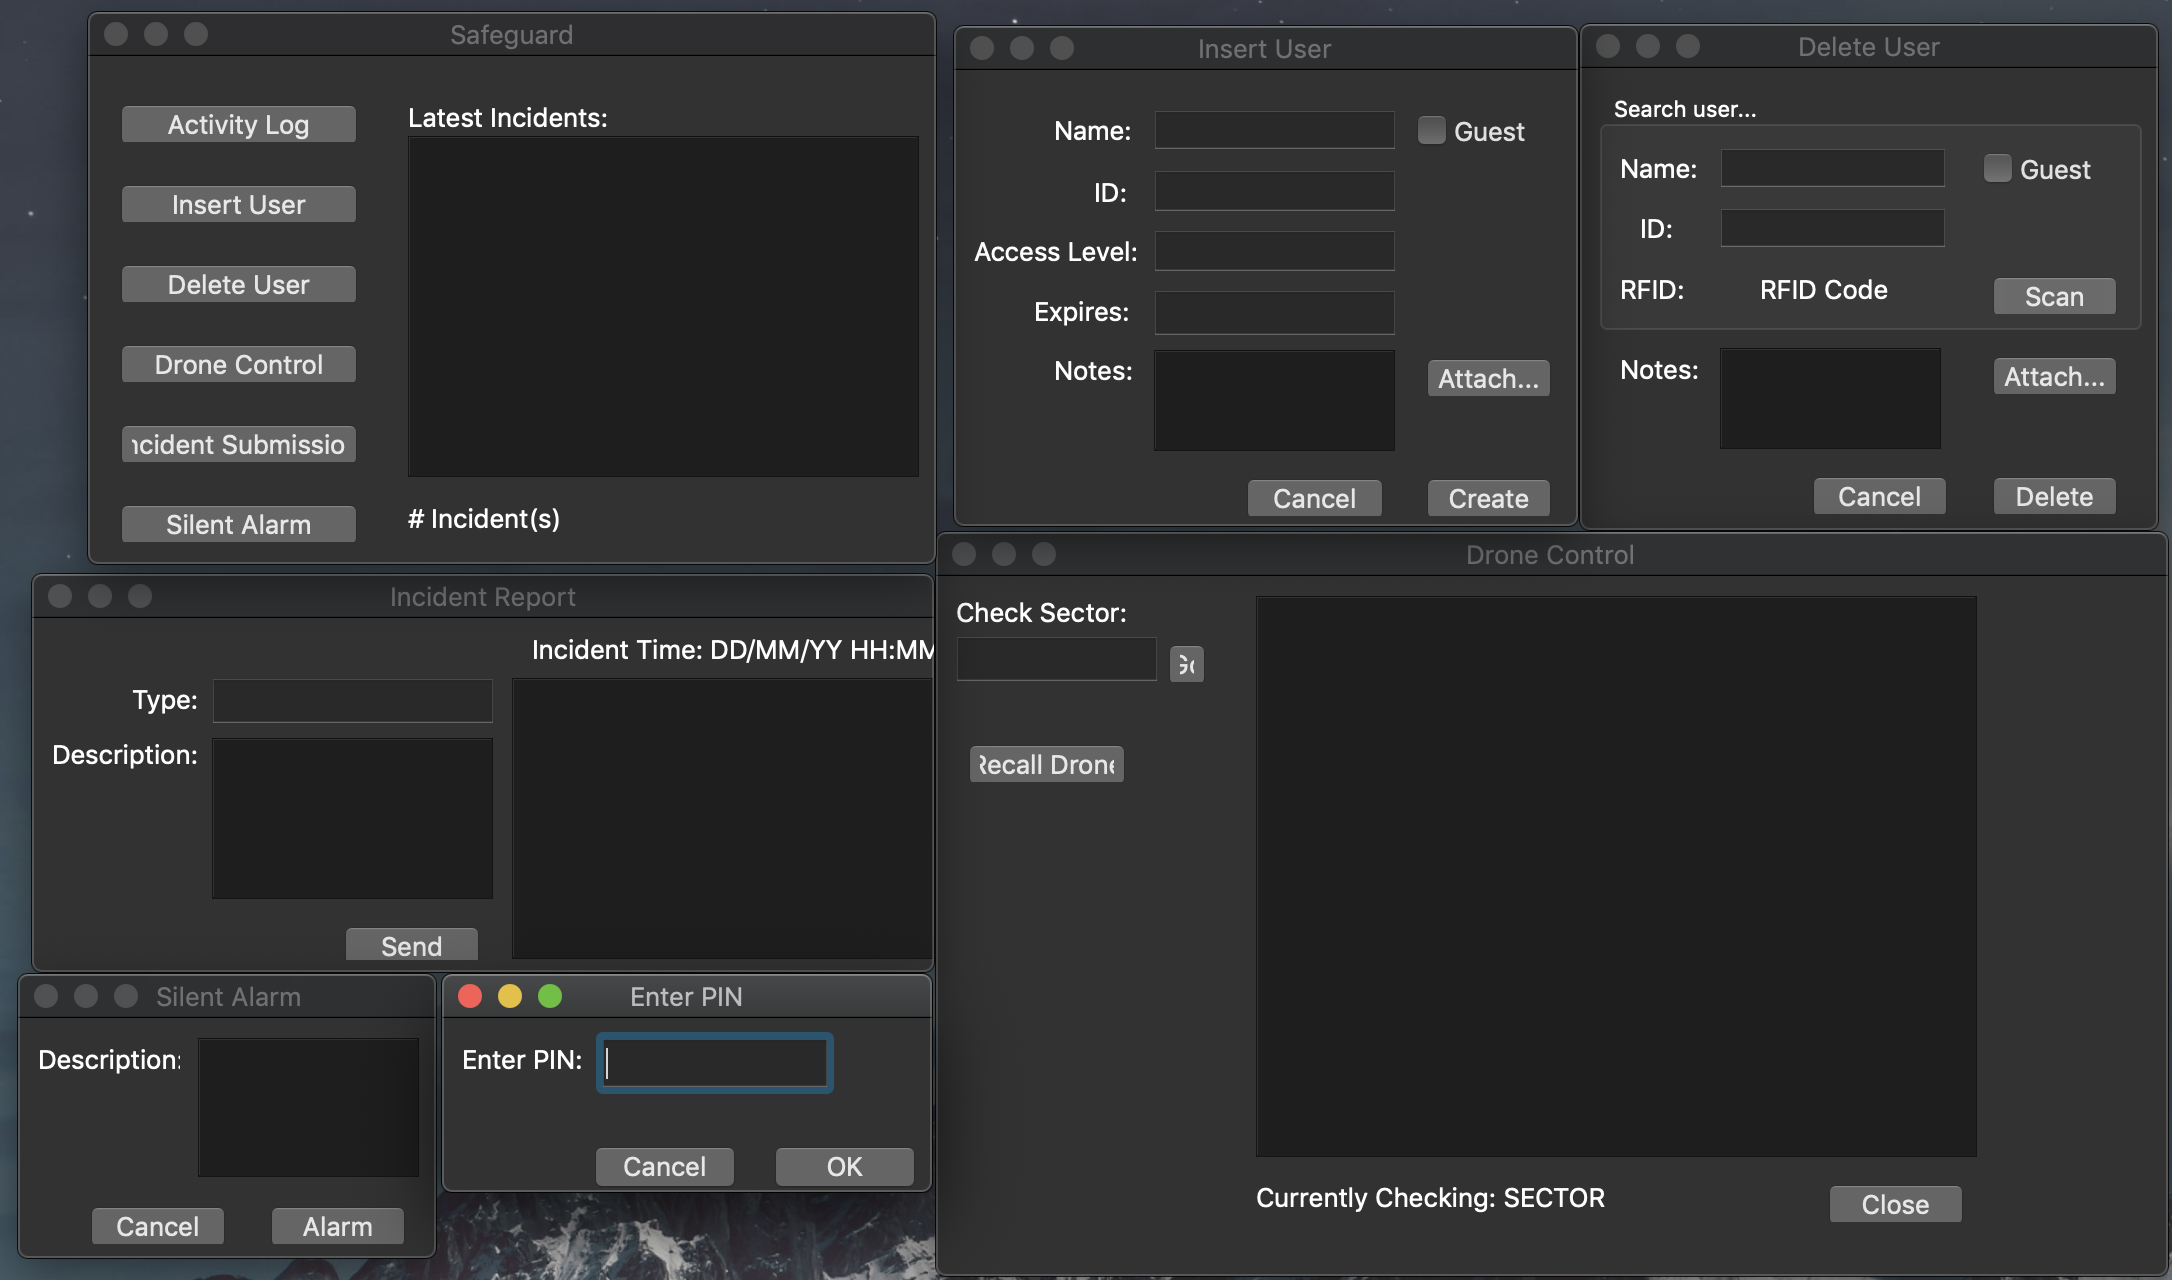
\includegraphics[width=0.9\paperwidth]{sweng_ui.png}}
\end{center}

\begin{center}
  \makebox[\textwidth]{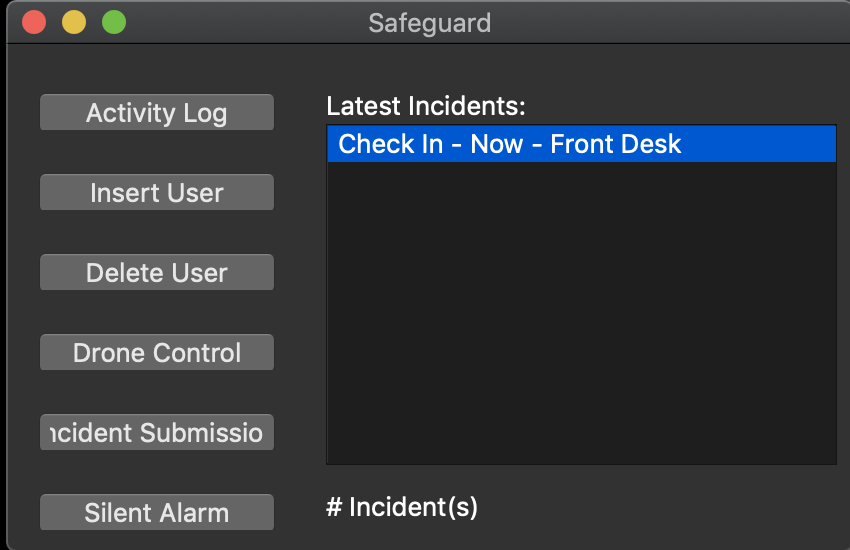
\includegraphics[width=0.9\paperwidth]{add_notif_incident.png}}
\end{center}

\begin{center}
  \makebox[\textwidth]{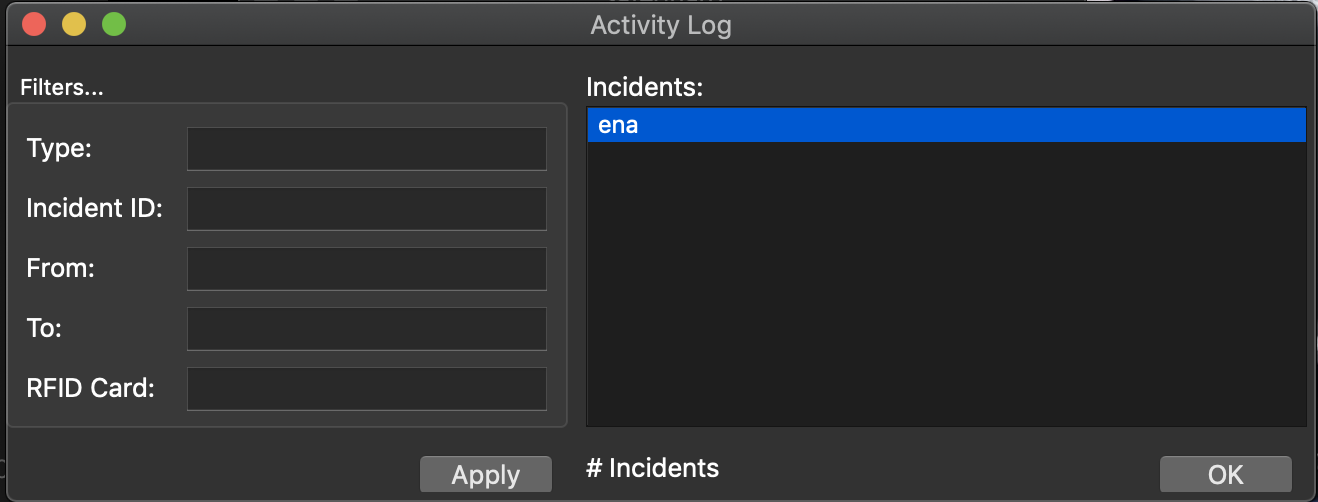
\includegraphics[width=0.9\paperwidth]{access_log.png}}
\end{center}

\section{Εργαλεία}
Χρησιμοποιήθηκαν:
\begin{itemize}
    \item \LaTeX/Overleaf.com - Συγγραφή του παρόντος τεχνικού κειμένου
    \item Photoshop - Φωτογραφία Σελίδας Τίτλου
    \item Qt Creator - UI Prototypes
    \item draw.io - Mock Up Wireframes
\end{itemize}


\end{document}
